\documentclass{article} % lub inna klasa dokumentu, np. report lub book
\usepackage[utf8]{inputenc} % ustawienie kodowania na UTF-8
\usepackage{amsmath, amssymb, amsthm} % biblioteki do działań matematycznych
\usepackage[T1]{fontenc}    % wybór odpowiedniego kodowania czcionek
\usepackage{polski}         % dodanie wsparcia dla polskich znaków
\usepackage{babel}          % automatyczne dostosowanie języka
\usepackage{pgfplots}       % Pakiet do tworzenia wykresów
\pgfplotsset{compat=1.18}

\title{Sprawozdanie}

\author{Tomasz Lisowski 197749\and Filip Świniarski 197725\and Nikodem Miłuch 197922}


\begin{document}
\maketitle
\section{Wstęp}
 
Celem ćwiczenia jest analiza ruchu drgającego prostego ciała zawieszonego na
sprężynie oraz wyznaczenie współczynnika sprężystości sprężyn i ich układów.

\subsection{Sprzęt laboratoryjny}

Do przeprowadzenia pomiarów wykorzystano m.in. wagę (podającą wynik do 0.001$kg$), zestaw sprężyn o różnych współczynnikach sprężystości $k$, stoper oraz linijkę z podziałką.

\section{Statyczne wyznaczanie współczynnika sprężystości}
\subsection{Opis doświadczenia}
Doświadczenie polega na wyznaczeniu współczynnika sprężystości sprężyny,  \\ wykorzystując zasadę Hooke’a. Na początku mierzymy długość sprężyny w jej spoczynkowym, nieobciążonym stanie. Następnie stopniowo zawieszamy na niej ciężarki o znanej masie, co powoduje jej wydłużenie. Po każdym dodaniu ciężarka mierzymy nową długość sprężyny i obliczamy przyrost jej długości względem początkowego stanu. Proces pomiarowy przebiegał następująco:
\begin{enumerate}
    \item Mierzymy długość sprężyny bez obciążenia i zapisujemy wynik.
    \item Stopniowo zawieszamy ciężarki o znanej masie ($m=0.05kg$) na końcu sprężyny.
    \item Po każdym dodaniu ciężarka mierzymy nową długość sprężyny.
\end{enumerate}

\subsection{Wyprowadzenie wzorów}

Z prawa Hook'a otrzymujemy gotowy wzór na współczynnik sprężystości $k$.
{\large
\begin{equation}
    F = k\Delta x
    \quad
    k = \frac{F}{\Delta x}
\end{equation}
}
Gdzie $\Delta x$ to bezwzględne wydłużenie sprężyny, a $F$ to wypadkowa siła działająca na układ. W naszym doświadczeniu:

{\large
\begin{equation}
    F = mg
\end{equation}
}

Gdzie $m$ to masa zawieszonych ciężarków, a $g$ to przyspieszenie ziemskie wynoszące ok. $9,81\frac{m}{s^2}$.

\subsection{Niepewność pomiarowa}

Niepewność pomiarowa $\Delta r$ jest równa najmniejszej możliwej odległości wyznaczonej za pomocą linijki. W tym przypadku $\Delta r = 0.001$m (1 mm). Masę ciężarków przyjmujemy za dokładną. Niepewność pomiarową wspołczynnika sprężystości. Na podstawie wykresu zależności $\Delta x$ od $m$ oraz wyników wyliczeń współczynnika kierunkowego przyjmujemy niepewność równą $\Delta r_k$ = 0.022 $\frac{m}{kg}$ . Do obliczeń wykorzystano przyspieszenie ziemskie wynoszące $g= 9,81\frac{m}{s^2}$.

\subsection{Wyniki pomiarów}

Wyniki pomiarów zebrano w Tabeli 1.
\begin{table}[h!]
\centering
\begin{tabular}{|c|c|c|c|}
\hline
\textbf{Lp.} & \textbf{Masa[$g$]} & \textbf{Wydłużenie[$cm$]}\\
\hline
1 & 0 & 0\\
2 & 50 & 3,5\\
3 & 100 & 7,2\\
4 & 150 & 10,6\\
5 & 200 & 14,2\\
6 & 250 & 17,8\\
\hline
\end{tabular}
\caption{Wyniki pomiarów}
\label{table:students}
\end{table}
\subsection{Wyniki doświadczenia}
Wyniki doświadczenia wraz z niepewnością pomiarową przedstawiono na wykresie poniżej. Niewność pomarowa wynosząca $\Delta r$ = 0.1 cm uwzględniona jest w rozmiarze punktów. Wspołczynnik kierunkowy wyznaczamy metodą graficzną korzystając z prawa Hook'a. Podstawiąjąc odpowiednie dane do wzoru (1) otrzymujemy.
{
\begin{center}
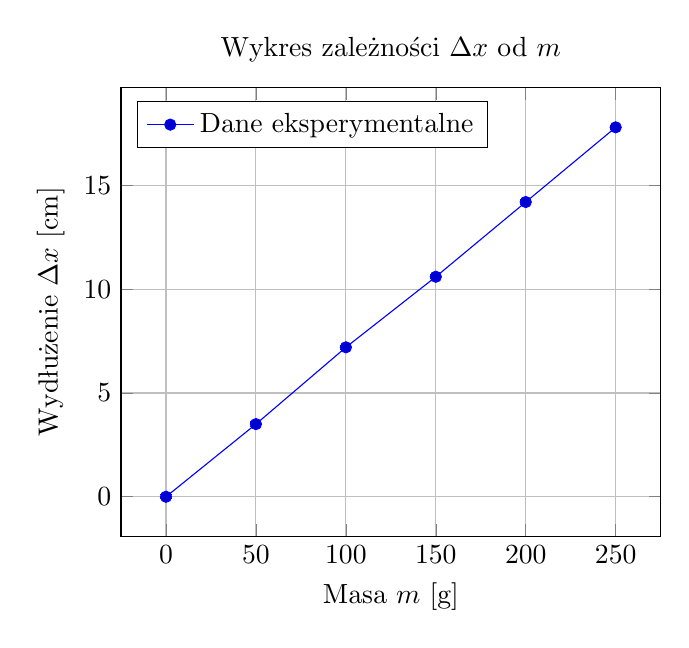
\begin{tikzpicture}
    \begin{axis}[
        ylabel={Wydłużenie $\Delta x$ [cm]}, % Etykieta osi X
        xlabel={Masa $m$ [g]},             % Etykieta osi Y
        grid=major,                        % Siatka na wykresie
        legend pos=north west,             % Pozycja legendy
        title={Wykres zależności $\Delta x$ od $m$}, % Tytuł wykresu
    ]
    \addplot+[
        mark=*,
        color=blue,
        error bars/.cd,
        y dir=both, % Enable error bars in both upward and downward directions
        y explicit % Explicitly define the errors
    ] coordinates {
        (0, 0.0) +- (0,0.1)
        (50, 3.5) +- (0,0.1)
        (100, 7.2) +- (0,0.1)
        (150, 10.6) +- (0,0.1)
        (200, 14.2) +- (0,0.1)
        (250, 17.8) +- (0,0.1)
    };
    \addlegendentry{Dane eksperymentalne}
    \end{axis}
\end{tikzpicture}



\begin{table}[h!]
\centering

\label{tab:coefficients}

\begin{tabular}{|c|c|}
\hline
\textbf{Masa \( m \) [kg]} & \textbf{Współczynnik kierunkowy \( k \) [m/kg]} \\ 
\hline
0.005 & 1.401 \\ 
0.010 & 1.360\\ 
0.015 & 1.388 \\ 
0.020 & 1.382 \\
0.025 & 1.379 \\
\hline
\end{tabular}
\caption{Współczynniki kierunkowe \( k \) dla każdego przedziału pomiarowego}
\end{table}
\end{center}
}
\subsection{Wyniki doświadczenia}

Uśredniając wyniki z Tabeli 2 otrzymujemy:
{\large
\begin{equation}
    k = 1.382 \pm0.022 \frac{m}{kg}
\end{equation}
}



\end{document}